\begin{frame}[t]
    \frametitle{Experimental Datasets}
    Tested on three datasets:\\
    \begin{itemize}
        \item SIFT100K: 1M rows with 128 dimensions of SIFT descriptors
        \item DEEP100K: 1B rows with 96 dimensions of image feature vectors
        \item GloVe100K: 400K rows with 300 dimensional GloVe vectors
    \end{itemize}

    All use 100,000 vectors as training queries and 10,000 as testing queries.
\end{frame}

\begin{frame}[t]
    \frametitle{Experiment Results}
    \begin{center}
        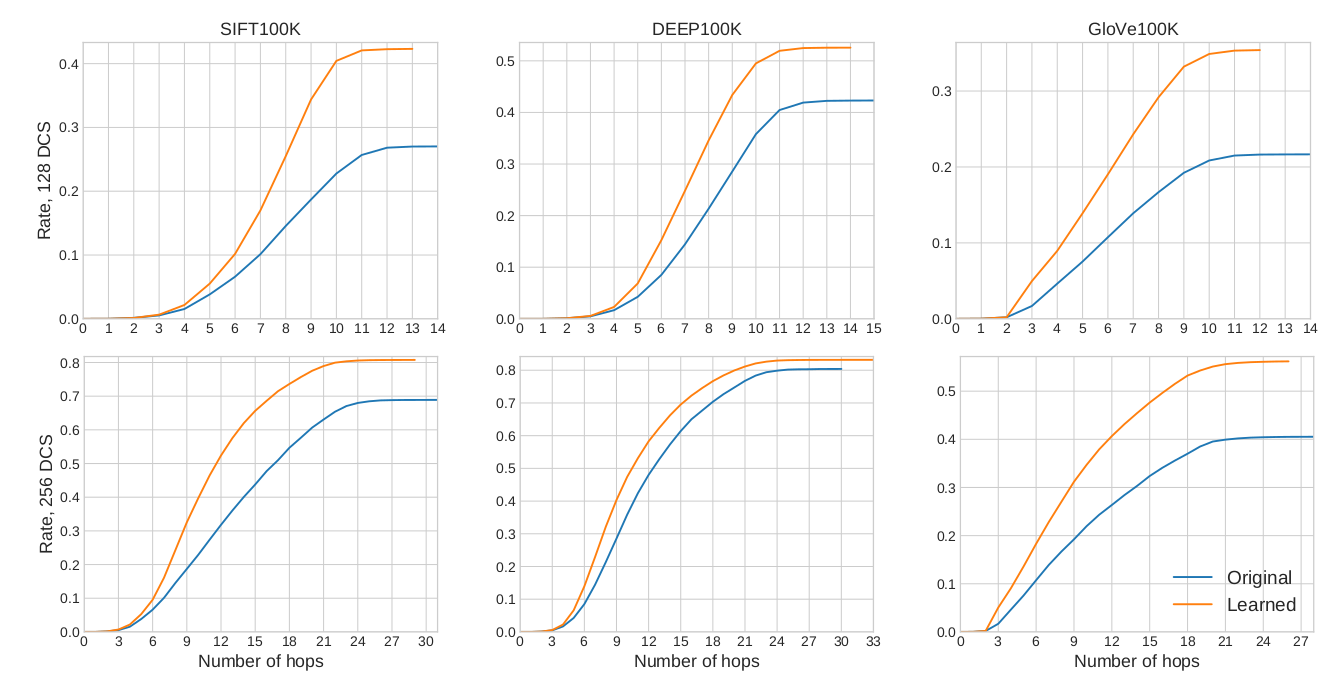
\includegraphics[width=30em, height=20em]{figures/Results1.png}
    \end{center}
\end{frame}

\begin{frame}[t]
    \frametitle{Experiment Results}
    Comparison between NNS solvers:\\
    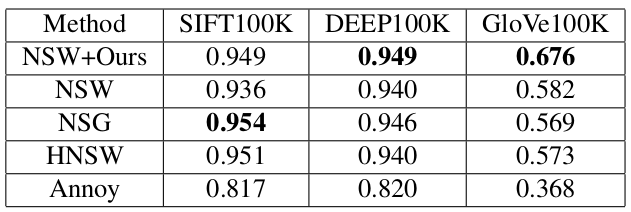
\includegraphics[scale=0.4]{figures/Results2.png}

    Note: Approach seems to work far better on high-dimensional data.

\end{frame}

\begin{frame}[t]
    \frametitle{Thank you!}
    Source: Learning to Route in Similarity Graphs by Baranchuk et al. (2019)\\
    \vspace{3.0em}
    Questions?

\end{frame}

% \begin{frame}{t}
%     \frametitle{Results: Model-Based Test}

%     \hspace{-2em}
% 	\begin{minipage}{0.49\textwidth}
% 		\begin{center}
%             Original Mapping:\\
% 			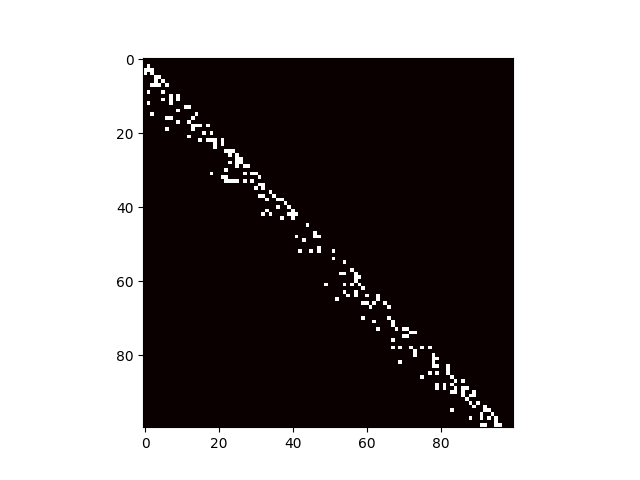
\includegraphics[scale=0.4]{figures/original_adj_100.png}
% 		\end{center}
% 	\end{minipage}
% 	\hspace{1em}
% 	\begin{minipage}{0.49\textwidth}
% 		\begin{center}
%             \hspace{0.1em} Gradient Descent:\\
% 			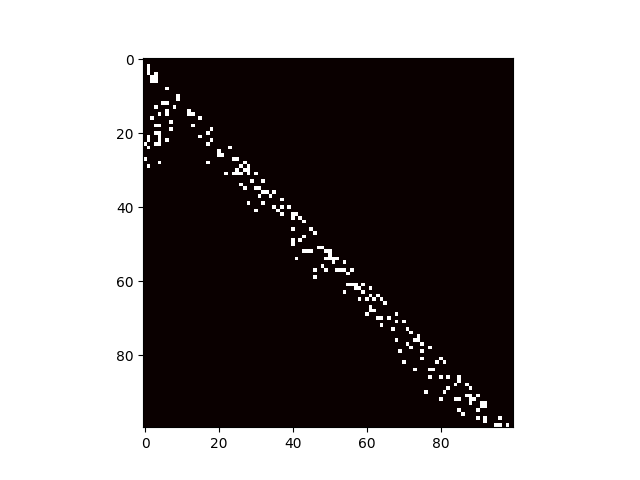
\includegraphics[scale=0.4]{figures/sgd_adj_100.png}
% 		\end{center}
% 	\end{minipage}
    
%     \onslide<2>{
%         Original Error: $\approx$1.2M\\
%         Gradient Descent Error: $\approx$1.6M
%     }

% \end{frame}

% \begin{frame}[t]
%     \frametitle{Results: On Real Data?}

%     \onslide<2-3>{
%         \begin{center}
%                 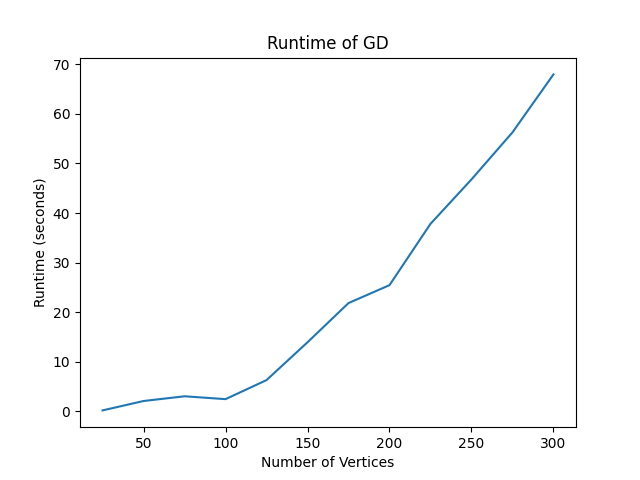
\includegraphics[scale=0.5]{figures/Runtime of Gradient Descent.png}
%         \end{center}
%     }

%     \onslide<3>{
%         Most large internet models have millions of vertices and \textbf{tens of millions} of edges.\\
%         This is nowhere near feasible on large graphs!
%     }
% \end{frame}

% \begin{frame}[t]
%     \frametitle{Next Steps}

%     \begin{itemize}
%         \item Investigate into applying fourier transforms
%         \item Find smaller dataset applications
%         \item Experiment with parameters of gradient descent
%     \end{itemize}
% \end{frame}

% \begin{frame}[t]
%     \frametitle{Thank you!}
%     Questions?
% \end{frame}